\section{Módulo anticheat.c: Monitoreo de acceso a archivos usando kprobe}

\subsection{Introducción y objetivo}

El archivo \texttt{anticheat.c} implementa un \textbf{módulo de kernel de Linux} diseñado para monitorear los intentos de acceso a un archivo específico en el sistema, simulando una funcionalidad básica de anti-cheat o protección. El objetivo es demostrar cómo los módulos de kernel pueden intervenir en operaciones sensibles y evidenciar la importancia de la seguridad al cargar módulos.

\subsection{¿Qué es \texttt{kprobe}?}

\texttt{kprobe} (kernel probe) es una interfaz del kernel de Linux que permite interceptar la ejecución de cualquier función interna del kernel, de forma dinámica y sin necesidad de recompilarlo. Al registrar un kprobe sobre una función, se puede ejecutar un ``handler'' (callback) personalizado cada vez que esa función es llamada.

En este contexto, kprobes se utiliza para \textbf{monitorear la apertura de archivos} mediante la interceptación de funciones como \texttt{do\_sys\_openat2} o \texttt{ksys\_openat}, que son responsables de manejar las llamadas \texttt{open()} y \texttt{openat()} en el kernel. Esta técnica es comúnmente empleada para debugging, profiling y tareas de monitoreo o seguridad.

\subsection{Descripción del funcionamiento}

El módulo \texttt{anticheat.c} registra un kprobe sobre la función interna del kernel encargada de abrir archivos. Cada vez que cualquier proceso intenta abrir un archivo, el handler del kprobe compara el nombre del archivo con una ruta específica (en este caso, \texttt{/tmp/trampa.txt}). Si coincide, el módulo imprime un mensaje de advertencia en el log del kernel, indicando el intento de acceso y el \texttt{PID} del proceso.

\begin{itemize}
    \item \textbf{No bloquea} el acceso: sólo lo detecta y lo registra para análisis.
    \item Es totalmente transparente para los programas de usuario.
    \item Demuestra el poder (y los riesgos) de los módulos para vigilancia y monitoreo a bajo nivel.
\end{itemize}
\newpage
\subsection{Código principal resumido}

\begin{verbatim}
/**
 * @file anticheat.c
 * @brief Módulo kernel: Monitorea acceso a archivo usando kprobe.
 * @author Tu Nombre
 */

#include <linux/module.h>
#include <linux/kernel.h>
#include <linux/kprobes.h>
#include <linux/uaccess.h>

#define FILE_MONITORED   "/tmp/trampa.txt"
#define PATH_LEN        128

static struct kprobe kp;

static int handler_pre(struct kprobe *p, struct pt_regs *regs)
{
    char filename[PATH_LEN] = {0};
#if defined(__x86_64__)
    char __user *user_filename = (char __user *)regs->si;
#elif defined(__aarch64__)
    char __user *user_filename = (char __user *)regs->regs[1];
#else
    #error "Arquitectura no soportada por este ejemplo"
#endif

    if (user_filename) {
        if (strncpy_from_user(filename, user_filename, PATH_LEN) > 0) {
            if (strcmp(filename, FILE_MONITORED) == 0) {
                printk(KERN_WARNING "[anticheat] Intento de abrir '%s' por PID %d (%s)\n",
                       filename, current->pid, current->comm);
            }
        }
    }
    return 0;
}

static int __init ac_init(void)
{
    kp.symbol_name = "do_sys_openat2";
    kp.pre_handler = handler_pre;
    register_kprobe(&kp);
    printk(KERN_INFO "[anticheat] Módulo cargado.\n");
    return 0;
}

static void __exit ac_exit(void)
{
    unregister_kprobe(&kp);
    printk(KERN_INFO "[anticheat] Módulo descargado.\n");
}

module_init(ac_init);
module_exit(ac_exit);

MODULE_LICENSE("GPL");
MODULE_AUTHOR("Tu Nombre");
MODULE_DESCRIPTION("Logger de intentos de apertura de archivo específico usando kprobe");
\end{verbatim}

\subsection{Funcionamiento y pruebas}

\begin{enumerate}
    \item \textbf{Compilación:} 
    \begin{verbatim}
    make
    \end{verbatim}
    \item \textbf{Carga del módulo:}
    \begin{verbatim}
    sudo insmod anticheat.ko
    \end{verbatim}
    \item \textbf{Prueba:} 
    Ejecutar cualquier comando que intente abrir el archivo monitoreado:
    \begin{verbatim}
    cat /tmp/trampa.txt
    \end{verbatim}
    \item \textbf{Ver logs del kernel:}
    \begin{verbatim}
    dmesg | tail
    \end{verbatim}
    Se verá una línea como:
    \begin{verbatim}
    [anticheat] Intento de abrir '/tmp/trampa.txt' por PID 12345 (cat)
    \end{verbatim}
    \item \textbf{Descarga del módulo:}
    \begin{verbatim}
    sudo rmmod anticheat
    \end{verbatim}
\end{enumerate}
\newpage
La siguiente imagen muestra el log del kernel sobre el intento de usar cat en trampa.txt

\begin{figure}[h!]
  \centering
  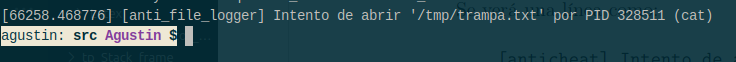
\includegraphics[width=0.8\linewidth]{images/dmesg.png}
  \caption{Log kernel por 'cat'}
\end{figure}

